\documentclass[10pt]{article}

\usepackage{amsmath}
\usepackage{relsize}
\usepackage{amssymb}
\usepackage{amsthm}
\usepackage{stmaryrd}
\usepackage{cancel}
\usepackage{wasysym}
\usepackage[usenames,dvipsnames]{color}
\usepackage{xspace}
\usepackage{url}
\usepackage{verbatim}
\usepackage{proof}
\usepackage{fullpage}
\usepackage{xr-hyper}
\usepackage[colorlinks,urlcolor=MidnightBlue,linkcolor=MidnightBlue,citecolor=MidnightBlue,backref]{hyperref}
\newcommand{\tab}{\hspace*{2em}}
\usepackage{graphicx}
\usepackage{amsmath}
\usepackage{newlfont}
\usepackage{listings}
\usepackage{pgf}
\usepackage{tikz}
\usepackage[latin1]{inputenc}
\usepackage{multicol}
\usetikzlibrary{arrows,automata,shapes}


\title{HW 6}
\author{Ross Yeager}
\date{May 14, 2013}
\begin{document}
\setlength\parindent{0pt}
\maketitle



%%%%%%%%%%%%%%%%%%%%%%%%%%%%%%%%%%%%%%%%%%%%%%%%%%%%%%

\section*{Exercise 1}


Suppose that whether or not it rains today depends on the previous weather conditions during
the last two days:\\

\begin{itemize}
\item If it has rained for the past two days, then it will rain tomorrow with probability 0:7.
\item If it rained today but not yesterday, then it will rain tomorrow with probability 0:5.
\item If it rained yesterday but not today, then it will rain tomorrow with probability 0:4.
\item If it has not rained in the past two days, then it will rain tomorrow with probability 0:2.
\end{itemize}


\subsection*{a)}

All outputs from each state sum up to be 1, a necessary requirement of a Markovian process; 
however, this system is not inheritely a Markov chain because a MC requires that what the next state depends only on the current state.  
In this process, weather depends on the weather today and yesterday. 
However, by simply redefining states as both the weather that day and the previous day.it can be made Markovian process with 4 states.\\

This process can be modelled as seen below with four states (RD denotes Rained yesterday, Dry today):\\
STATES:
\begin{itemize}
\item RR
\item DR
\item RD
\item DD
\end{itemize}


\begin{multicols}{2}
\begin{tikzpicture}[->,>=stealth',shorten >=1pt,auto,node distance=2cm]
\tikzstyle{every state}=[fill=none,draw=black,text=black]
\node[state] (A)        {$RR$};
\node[state] (B) [right of=A] {$DR$};
\node[state] (C) [right of=B] {$RD$};
\node[state] (D) [right of=C] {$DD$};
\path   (A)     edge [bend right] node[yshift = -.45cm] {0.3} (C)
                edge [loop above] node{0.7} (A)
        (B)     edge [bend left] node {0.5} (C)
                edge node [yshift=0.45cm] {0.5} (A)
        (C)     edge [bend left] node[yshift = 0.45cm] {0.4} (B)
                edge [bend right] node[below]  {0.6} (D)
        (D)     edge [loop above] node {0.8} (D)
                edge [bend right] node[above] {0.2} (C)
\end{tikzpicture}

\[
P = 
\left[
\begin{array}{c|cccc}
   & RR & DR & RD & DD \\ \hline 
RR & 0.7 & 0 & 0.3 & 0 \\
DR & 0.5 & 0 & 0.5 & 0 \\
RD & 0 & 0.4 & 0 & 0.6 \\
DD & 0 & 0.2 & 0 & 0.8
\end{array}
\right]
\]
\end{multicols}
\subsection*{b)}

\begin{itemize}
\item The resulting Markov Chain is finite.
\item The resulting Markov Chain is irreducible since all states are accessable from all states.
\end{itemize}


\subsection*{c)}

The resulting Markov Chain has the following probability matrix, $P$:

\[
P = 
\left[
\begin{array}{c|cccc}
   & RR & DR & RD & DD \\ \hline 
RR & 0.7 & 0 & 0.3 & 0 \\
DR & 0.5 & 0 & 0.5 & 0 \\
RD & 0 & 0.4 & 0 & 0.6 \\
DD & 0 & 0.2 & 0 & 0.8
\end{array}
\right]
\]

Because the MC is finite and irreducible, it must have a stationary distribution.  This matrix does converge as $k\rightarrow \infty$, therefore it does have a stationary distribution. For example, $P^{100}$ results in

\begin{center}
\[
$P^{100} =$ 
\left[
\begin{array}{c c c c}
0.2500 & 0.1500 & 0.1500 & 0.4500 \\
0.2500 & 0.1500 & 0.1500 & 0.4500 \\
0.2500 & 0.1500 & 0.1500 & 0.4500 \\
0.2500 & 0.1500 & 0.1500 & 0.4500 
\end{array}
\right]
\]
\end{center}

The resulting stationary distribution is 

\begin{equation*}
\pi = [0.25, 0.15, 0.15, 0.45]
\end{equation*}
%%%%%%%%%%%%%%%%%%%%%%%%%%%%%%%%%%%%%%%%%%%%%%%%%%%%%%

\section*{Exercise 2}

\subsection*{a)}

Screenshots from the designed electronic circuit:\\\\


Circuit: \\
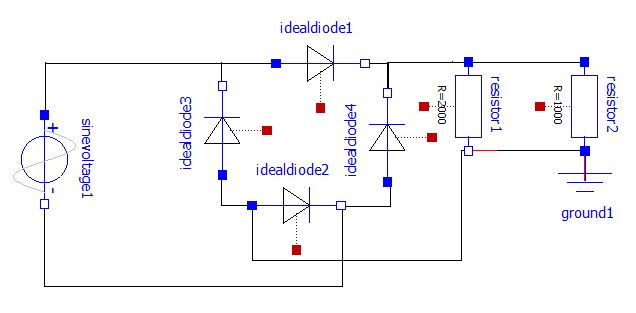
\includegraphics[width=0.8\textwidth]{ModelicaModel.JPG}\\

Simulation: \\

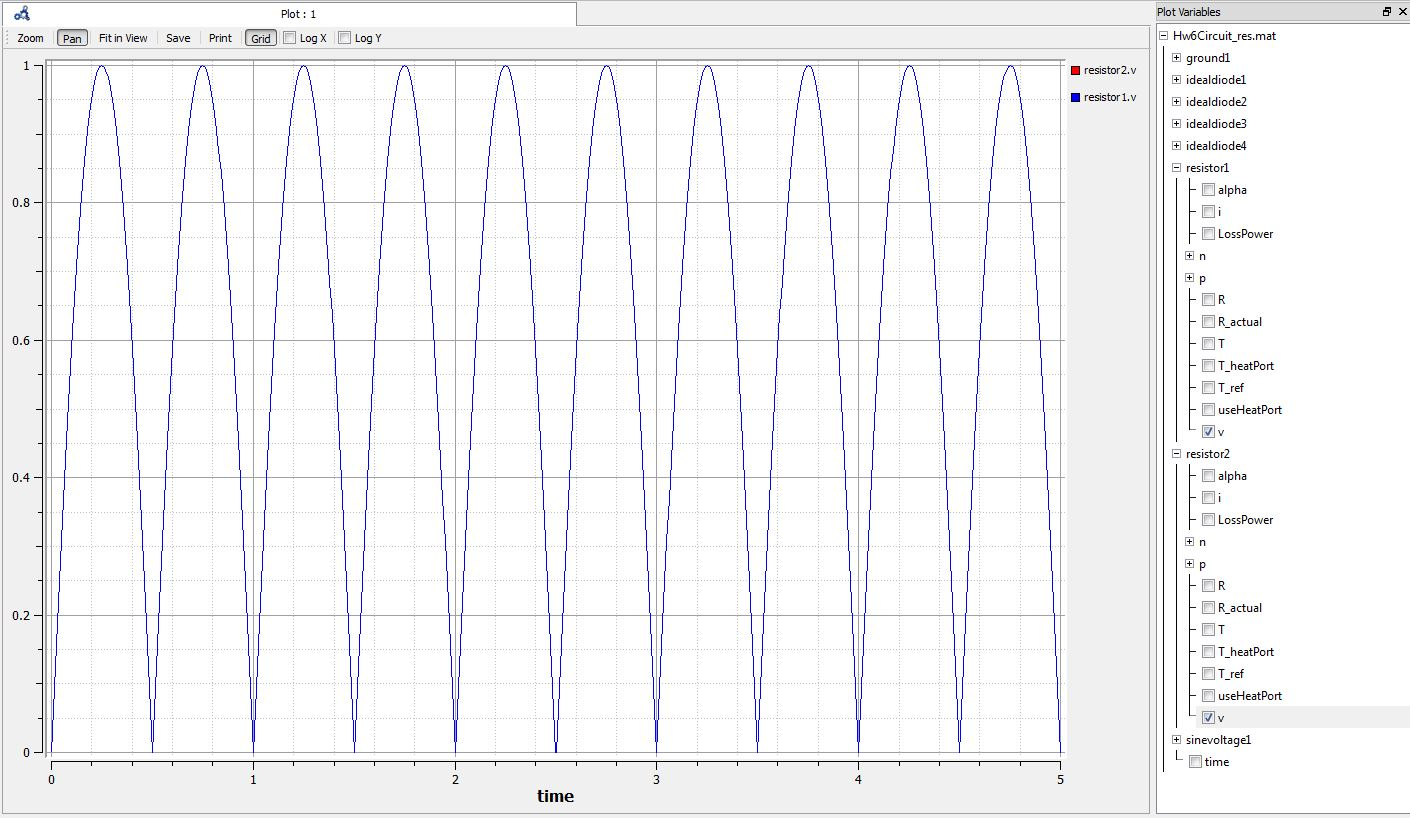
\includegraphics[width=0.8\textwidth]{fullwaverectifier.JPG}\\


\subsection*{b)}

This circuit design is that of a full wave rectifier.  It contains 4 diodes, an AC source, and two "loads" represented here as resistors in parallel.  The output across the loads is a rectified A/C signal, i.e. the signal is all positive from a periodic sinosoidal source signal.  A capacitor can be thrown across the load to effectively convert the AC signal to a DC signal.  The reverse biased diodes are what ensure that the signal is always positive.  The resistor values are 2k Ohm and 1k Ohm (the voltage across them both will be the same since they are in parallel).  The voltage across the loads can be seen below in $c)$.

\subsection*{c)}

\lstinputlisting{hw6.txt}


%%%%%%%%%%%%%%%%%%%%%%%%%%%%%%%%%%%%%%%%%%%%%%%%%%%%%%

\section*{Exercise 3}

\subsection*{a)}

Examining the given system of differntial algebraic equations: \\
\textbf{Variables: ($x_1, x_2, x_3, y_1, y_2, y_3$)}\\
\textbf{Differentiated: ($\dot y_1, \do y_2$)}\\

\[
M_i = 
\left[
\begin{array}{c|cccccc}
   & \dot y_1  & \dot y_2 & y_3 & x_1  & x_2 & x_3 \\ \hline 
f_1 &  1 & 0 & 0 & 1 & 0 & 0 \\
f_2 &  0 & 1 & 0 & 0 & 1 & 0 \\
f_3 &  0 & 0 & 1 & 0 & 0 & 1 \\
f_4 &  0 & 0 & 1 & 0 & 0 & 0 \\
f_5 &  0 & 0 & 0 & 0 & 0 & 0 \\
f_6 &  0 & 0 & 0 & 1 & 1 & 1 \\
\end{array}
\right]
\]


\subsection*{b)}

The BLT sorting algorithm does not succeed.  This is because of equation 5, which has zero entries for all differentiated and algebraic variables and therefore there are only 5 relations for 6 variables.

\subsection*{c)}

Now we assume that equation $(5)$ is differentiated and replaced with this new equation: \\

\begin{equation*}
\dot y_1 = \dot y_2 (5)
\end{equation*}

Now the BLT sorting algorithm can be applied again.  

This allows for the successful implementation of the algorithm, with a successfully sorted incidence matrix, $M_i$:
\[
M_i = 
\left[
\begin{array}{c|cccccc}
   & \dot y_1  & \dot y_2 & y_3 & x_1  & x_2 & x_3 \\ \hline 
f_1 &  1 & 0 & 0 & 1 & 0 & 0 \\
f_2 &  0 & 1 & 0 & 0 & 1 & 0 \\
f_3 &  0 & 0 & 1 & 0 & 0 & 1 \\
f_4 &  0 & 0 & 1 & 0 & 0 & 0 \\
f_5 &  1 & 1 & 0 & 0 & 0 & 0 \\
f_6 &  0 & 0 & 0 & 1 & 1 & 1 \\
\end{array}
\right]
\]


\subsection*{d)}

Yes, this new DAE has algebraic loops.  The involved equations are:

\begin{equation*}
equation here
\end{equation*}

\subsection*{e)}

The index of the sorted system in step $(c)$ is of index 1.

%%%%%%%%%%%%%%%%%%%%%%%%%%%%%%%%%%%%%%%%%%%%%%%%%%%%%%
\end{document}
